\chapter*{Abstract}
\phantomsection
\addcontentsline{toc}{chapter}{Abstract}%
\markboth{Abstract}{Abstract}%
todo

\newpage
\chapter*{Introduction}
\phantomsection
\addcontentsline{toc}{chapter}{Introduction}
\markboth{Introduction}{Introduction}%


\textit{Scientists study the world as it is,}\\
\textit{Engineers create the world that never has been.} \vspace{5pt} \\
--- Theodore von K\'arm\'an \\

\section*{Towards lighter structures}

In the aerospace industry, an ongoing demand exists for lighter aerostructures, motivated by the need to enhance fuel efficiency and overall performance. This emphasis on lighter structures and materials not only reduces operational costs for airlines but also aligns with a broader commitment to sustainability, mitigating fuel consumption and carbon emissions. Furthermore, the aerospace sector is currently witnessing two innovative shifts: the transition to hydrogen-powered and electric planes, directing engineering efforts toward cleaner and more sustainable aviation technologies. These changes offer opportunities to deviate from the classic tube-and-wing configuration and explore inventive concepts like the flying wing \gls{bwb}, in which the fuselage and the wing blend together to form an aircraft in which the fuselage, widened and integrated into the wing, also contributes significantly to the lift, or transonic truss-braced wings, with the goal of direct reduction in the aerodynamic drag by using a high-aspect ratio strut-braced wing configuration (see examples in \figref{fig:01_concepts}). Regardless of the specific configuration, a highly probable shared goal is the necessity to redesign lightweight dry--\ie with no fuel tanks inside--wings with high aspect ratios and thin profiles.

\begin{figure*}
    \hspace*{\fill}
    \subcaptionbox{}{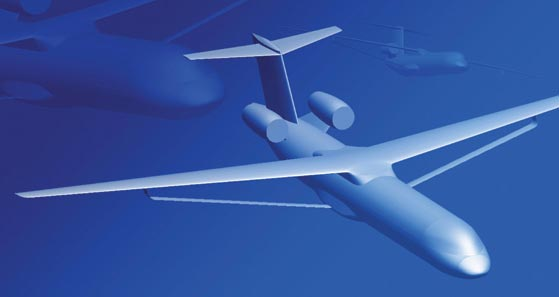
\includegraphics[height=4.3cm]{figures/01_intro/albatros-1.jpg}}
    \hfill
    \subcaptionbox{}{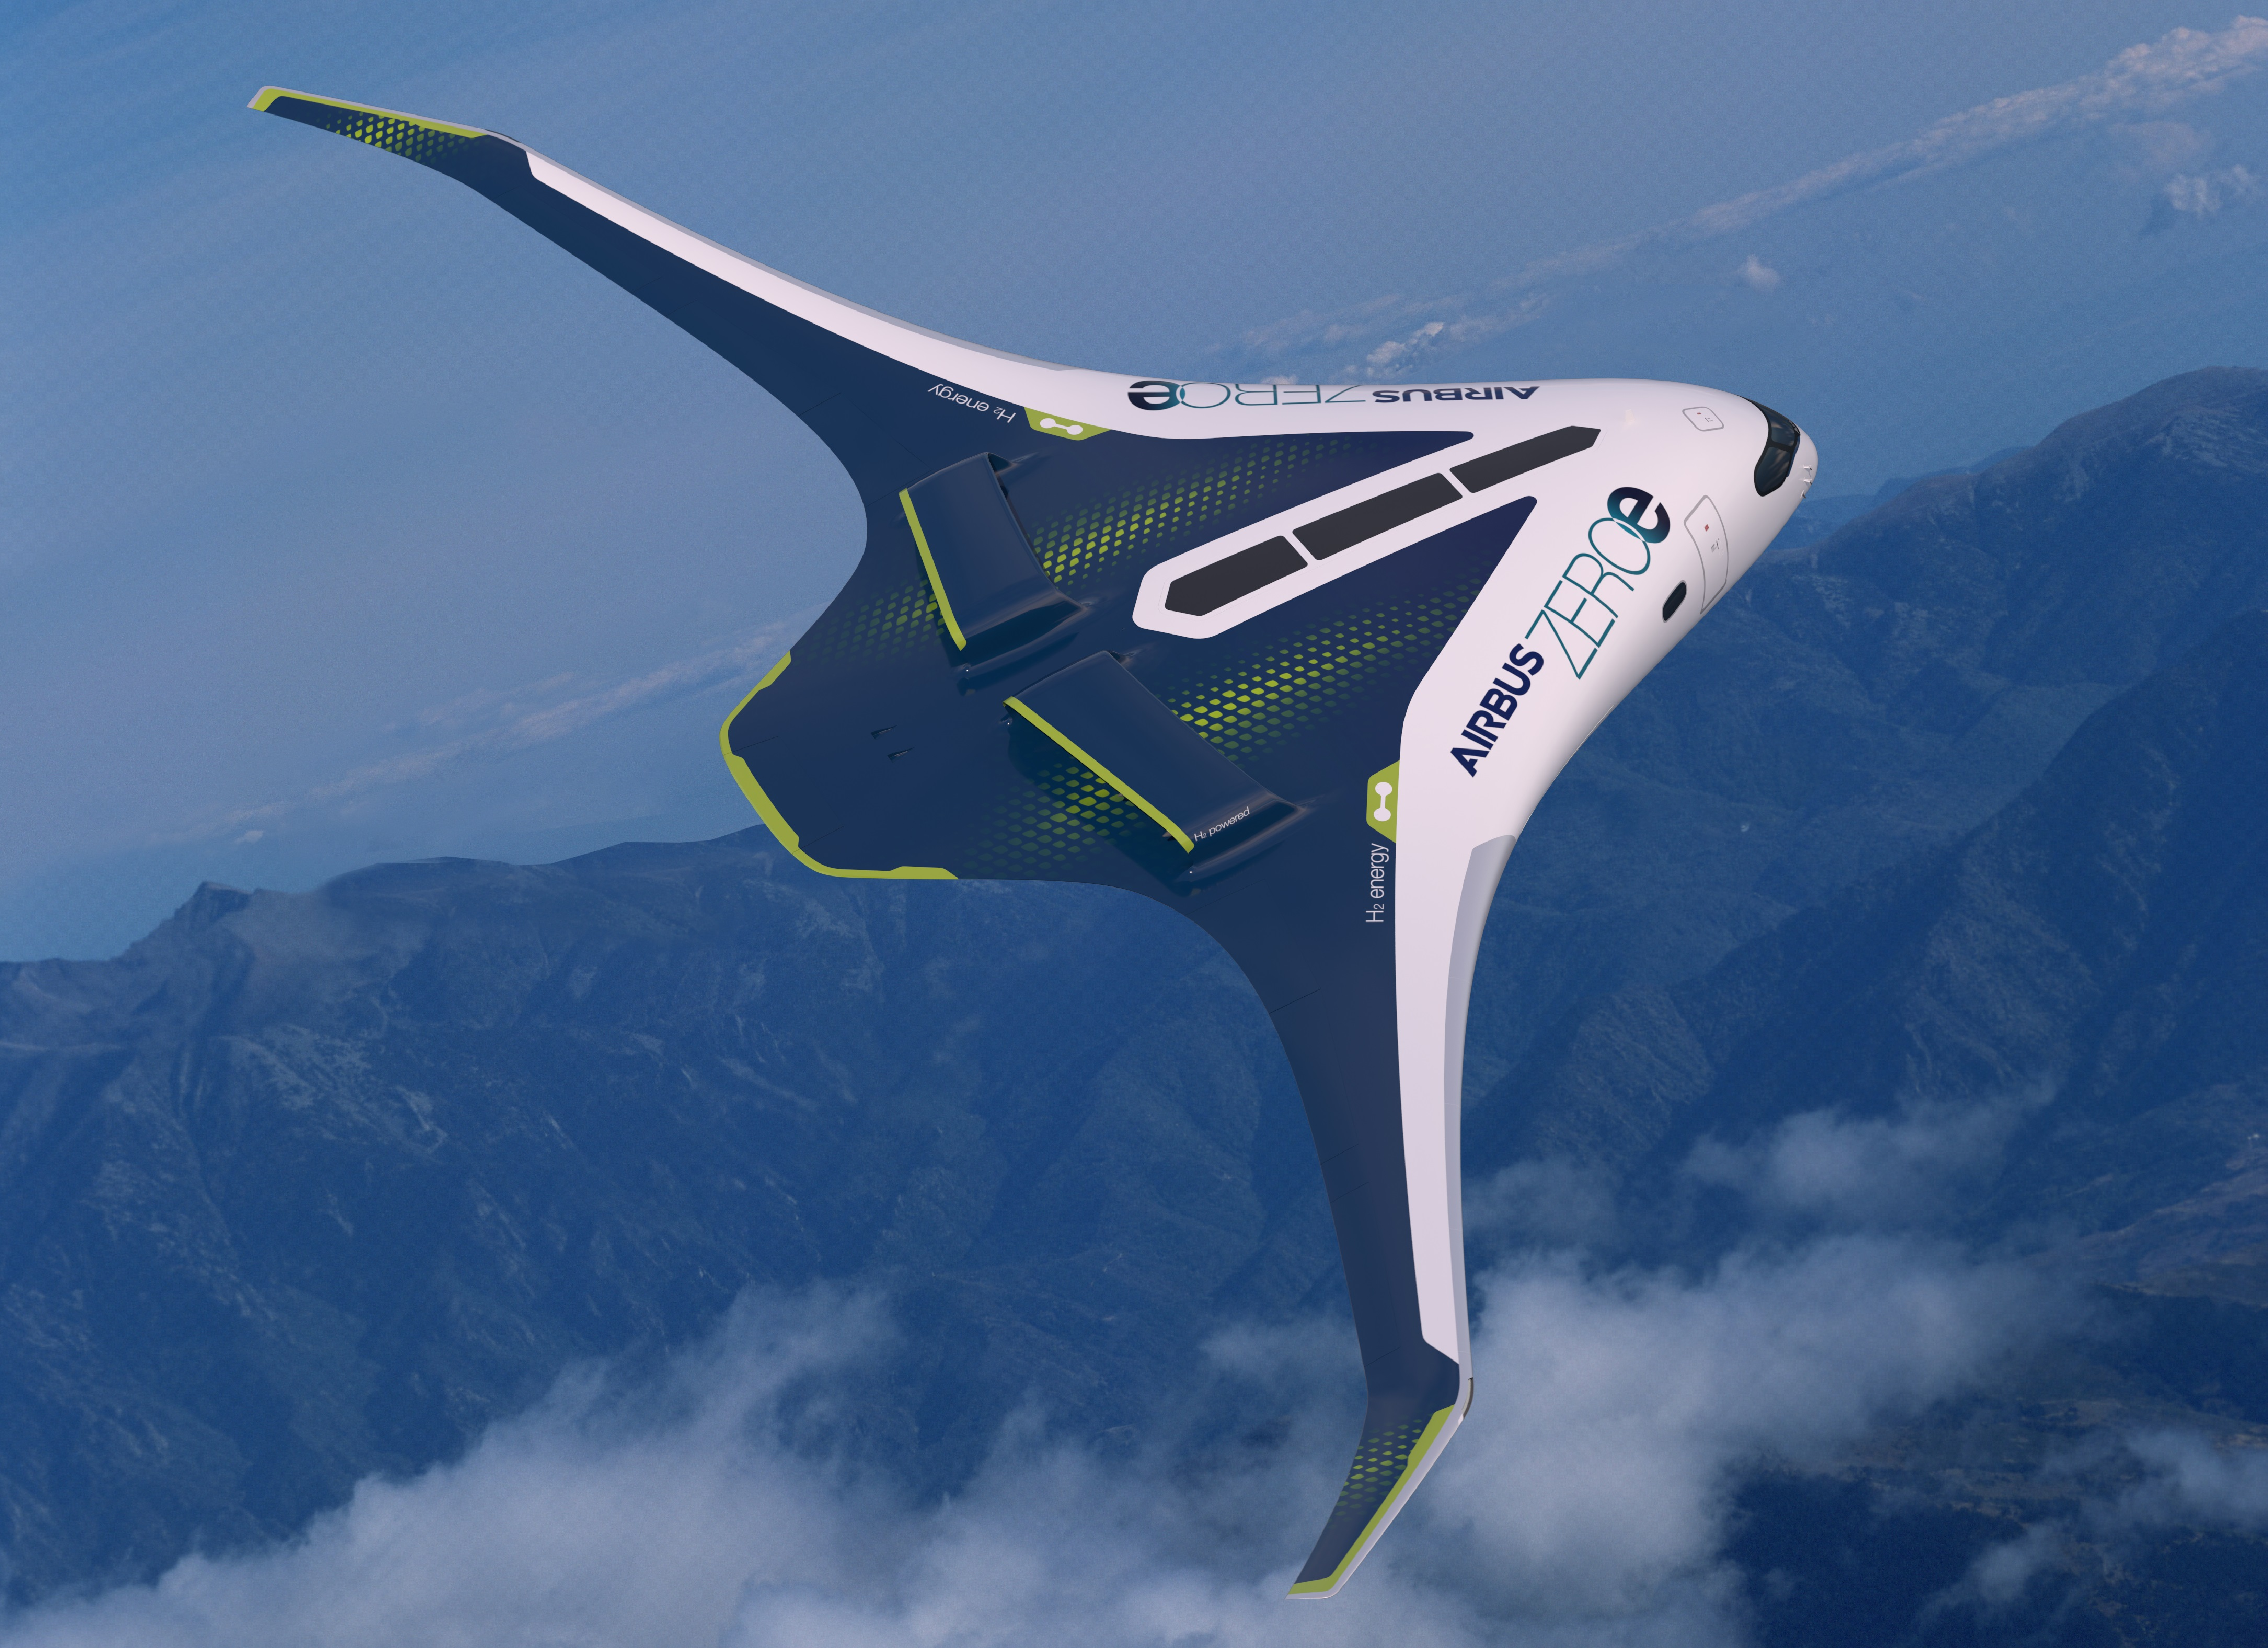
\includegraphics[height=4.3cm]{figures/01_intro/pm_38_529_529759-gml5anffhc.jpg}}
    \hspace*{\fill}
    \caption{(a) The transonic truss-braced wing called ALBATROS by ONERA \cite{carrier_investigation_2012,carrier_multidisciplinary_2021}; (b) the \acrfull{bwb} zero-e demonstrator by Airbus \cite{noauthor_airbus_2021}.}
    \label{fig:01_concepts}
\end{figure*}

To meet these criteria, a promising solution involves the application of lattice structures. Not only do these structures provide the necessary ultralight properties, but they also offer modularity. Modular designs come with several advantages, notably the capability to construct large structures using smaller, more easily manufactured repeating modules. Other notable properties include on-field reparability, improved damage resistance, fast assembly for temporary structures, and stochastic error detection and repair compared to conventional monolithic material systems \sidecite{belvin_space_2016}. Additionally, recent research opens up the possibility of a fully robotic assembly phase, permitting faster and more reliable assembly (see \figref{fig:01_fab}).

\begin{figure}
    \hspace*{\fill}
    \subcaptionbox{}{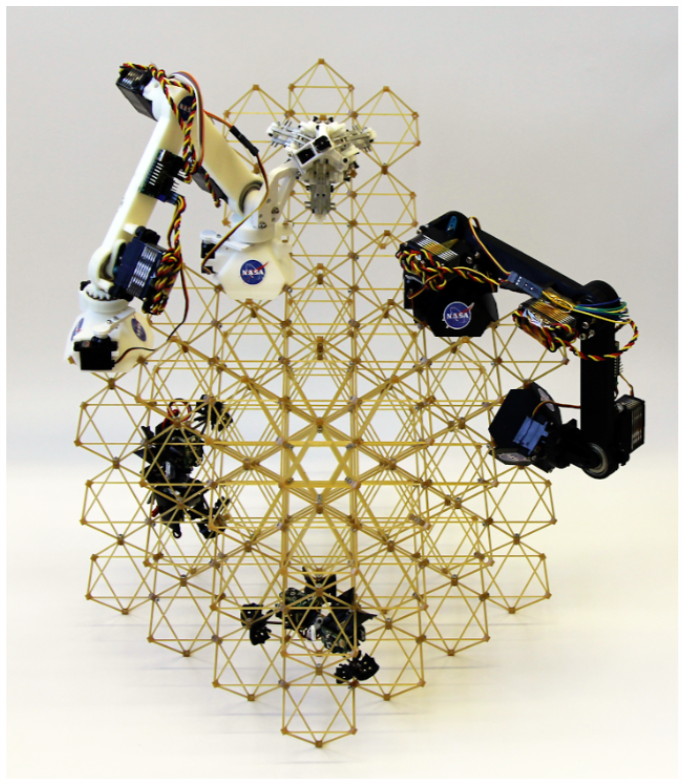
\includegraphics[height=3.5cm]{figures/01_intro/fab.png}}
    \hfill
    \subcaptionbox{}{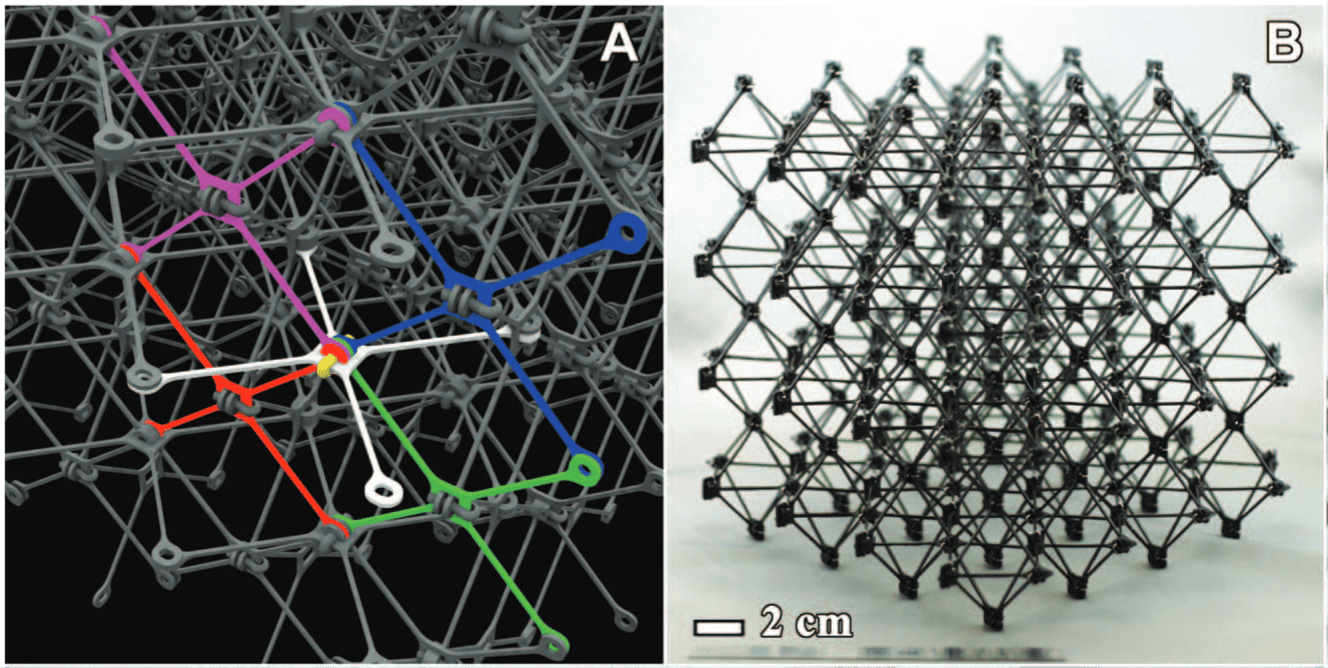
\includegraphics[height=3.5cm]{figures/01_intro/assembly.png}}
    \hspace*{\fill}
    \caption{\cite{cheung_reversibly_2013} \cite{costa_algorithmic_2020}.}
    \label{fig:01_fab}
\end{figure}

Optimizing lattice structures involves four main dimensions: material, module shape, layout, and topology. Material optimization focuses on improving mechanical properties by tailoring the distribution of lattice constituents, while shape optimization fine-tunes individual module external geometries. Layout optimization arranges modules in space, defining their presence or absence, and topology optimization refines overall arrangement and connections within each module. Navigating these dimensions enables engineers to tailor lattice structures for a balance between weight, strength, and functionality. However, the abundance of design choices poses a significant challenge due to the lack of a standardized design method. Navigating this intricate landscape requires a systematic and efficient approach to ensure the resulting lattice structure meets specific engineering requirements. 

\section*{Objective}
This thesis aims to develop an optimization formulation and algorithm specifically designed for ultralight and modular aerostructures within the aerospace industry. In this field, reducing weight is crucial for improving overall performance. However, the introduction of modularity, while offering advantages such as manufacturing easing or improved damage resistance, may potentially lead to an increase in the overall weight of the structure when compared to classic monolithic structures. Consequently, the primary objective throughout this thesis is to develop an optimization method that not only harnesses the benefits of modularity but also ensures that the resultant structure remains as lightweight as possible. Striking a balance between the manufacturing advantages conferred by modularity and the critical need for weight reduction forms the central focus of this research.

\section*{Outline of the thesis}
The remainder of the thesis is structured as follows. \chpref{chap:02} provides a comprehensive review of structural optimization algorithms, especially focusing on ultralight weight and modular cases. The chapter introduces density-based topology optimization and the \gls{tto} formulations that will be utilized throughout the document. \chpref{chap:03} delves into a detailed comparison of the topology optimization methods, emphasizing results obtained when optimized structures exhibit a very low volume fraction, \ie less than \qty{5}{\percent}. A shared volume minimization with stress constraints formulation is presented, and a comparison is conducted by varying the material mechanical properties to achieve different volume fractions. After careful analysis, the \gls{tto} approach is selected due to its reduced computational time and suitability for modeling lightweight structures. \chpref{chap:04} addresses the limitations of the classic \gls{tto} formulation, such as the absence of local buckling constraints, minimum slenderness limits, consideration of multiple load cases, and ensuring mechanical compatibility for complex structures. To overcome these challenges, an innovative volume minimization formulation is proposed, incorporating the additional constraints needed to optimize real-world structures. Due to the inherent multimodality of the formulation, a two-step optimization algorithm is introduced, utilizing a relaxed problem to generate an initial approximate solution for subsequent optimization using a complete formulation. The Reinitialization heuristic is also proposed to reduce the influence of the starting point on optimization results. \chpref{chap:05} explores the incorporation of modular constraints in the proposed \gls{tto} formulation, employing the full-scale variable linking approach. This approach repeats a single module throughout the entire design to create optimized modular structures. The chapter evaluates the impact of hyperparameters, such as the number of subdomains and module complexity, on the mechanical performance of the structure. A Design of Experiments (\gls{doe}) based on the chapter's results provides guidance on choosing hyperparameters for optimization. In \chpref{chap:06}, the optimization scenario becomes more complex by introducing an additional optimization variable: the addition of multiple different topology modules. This optimization, inherently more complex, involves optimizing not only the modules' topology but also the layout of the modules within the structure. A modified \gls{dmo} approach is employed, utilizing a gradient-based optimizer, while the starting point is determined by employing k-means clustering on the stress distribution of the unoptimized initial structure. Up to this point, the focus has been on academic two or three-dimensional test cases. Chapter \chpref{chap:07} extends the application of the proposed optimization formulation and algorithms to the aerospace domain. Initially, the monolithic optimization algorithm is used to reduce the weight of the wingbox of the \gls{crm}, a standard benchmark for aeronautic research. The test case is subjected to multiple load cases(+2.5g, -1g and cruise loads) associated with some correspective safety factors. The optimization is conducted using different materials and discretizations, resulting in lighter structures in less time compared to the literature. Later, the modular optimization formulation presented in \chpref{chap:06} is used on a drone-sized wing based on the 0012 NACA wing profile. Additionally, follow-up scientific perspectives are discussed.